\documentclass[10pt,letterpaper]{article}
\usepackage[utf8]{inputenc}
\usepackage[intlimits]{amsmath}
\usepackage{amsfonts}
\usepackage{amssymb}
\usepackage{ragged2e}
\usepackage[letterpaper, margin=0.5in]{geometry}
\usepackage{graphicx}
\usepackage{cancel}
\usepackage{mathtools}
\usepackage{tabularx}
\usepackage{arydshln}
\usepackage{tensor}
\usepackage{array}
\usepackage{xcolor}
\usepackage[boxed]{algorithm}
\usepackage[noend]{algpseudocode}
\usepackage{listings}
\usepackage{textcomp}
% \usepackage[pdf,tmpdir,singlefile]{graphviz}
\usepackage{mathrsfs}
\usepackage{bbm}
\usepackage{tikz}
\usepackage{tikz-cd}
\usepackage{enumitem}
\usepackage{arydshln}
\usepackage{relsize}
\usepackage{multicol}
\usepackage{scalerel}
\usepackage{upgreek}
\usepackage{ifthen}

\usetikzlibrary{bayesnet}
\setlist{noitemsep}

%%%%%%%%%%%%%%%%%%%%%%%%%%%%%
% Formatting commands
%%%%%%%%%%%%%%%%%%%%%%%%%%%%%
\newcommand{\n}{\hfill\break}
\newcommand{\nn}{\vspace{0.5\baselineskip}\n}
\newcommand{\up}{\vspace{-\baselineskip}}
\newcommand{\hangblock}[2]{\par\noindent\settowidth{\hangindent}{\textbf{#1: }}\textbf{#1: }\nolinebreak#2}
\newcommand{\lemma}[1]{\hangblock{Lemma}{#1}}
\newcommand{\defn}[1]{\hangblock{Defn}{#1}}
\newcommand{\thm}[1]{\hangblock{Thm}{#1}}
\newcommand{\cor}[1]{\hangblock{Cor}{#1}}
\newcommand{\prop}[1]{\hangblock{Prop}{#1}}
\newcommand{\ex}[1]{\hangblock{Ex}{#1}}
\newcommand{\exer}[1]{\hangblock{Exer}{#1}}
\newcommand{\fact}[1]{\hangblock{Fact}{#1}}
\newcommand{\remark}[1]{\hangblock{Remark}{#1}}
\newcommand{\proven}{\;$\square$\n}
\newcommand{\problem}[1]{\par\noindent{\nolinebreak#1}\n}
\newcommand{\problempart}[2]{\par\noindent\indent{}\settowidth{\hangindent}{\textbf{(#1)} \indent{}}\textbf{(#1) }\nolinebreak#2\n}
\newcommand{\ptxt}[1]{\textrm{\textnormal{#1}}}
\newcommand{\inlineeq}[1]{\centerline{$\displaystyle #1$}}
\newcommand{\pageline}{\up\par\noindent\rule{\textwidth}{0.1pt}}

%%%%%%%%%%%%%%%%%%%%%%%%%%%%%
% Math commands
%%%%%%%%%%%%%%%%%%%%%%%%%%%%%
% Set Theory
\newcommand{\card}[1]{\left|#1\right|}
\newcommand{\set}[1]{\left\{#1\right\}}
\newcommand{\setmid}{\;\middle|\;}
\newcommand{\ps}[1]{\mathcal{P}\left(#1\right)}
\newcommand{\pfinite}[1]{\mathcal{P}^{\ptxt{finite}}\left(#1\right)}
\newcommand{\naturals}{\mathbb{N}}
\newcommand{\N}{\naturals}
\newcommand{\integers}{\mathbb{Z}}
\newcommand{\Z}{\integers}
\newcommand{\rationals}{\mathbb{Q}}
\newcommand{\Q}{\rationals}
\newcommand{\reals}{\mathbb{R}}
\newcommand{\R}{\reals}
\newcommand{\complex}{\mathbb{C}}
\newcommand{\C}{\complex}
\newcommand{\halfPlane}{\mathbb{H}}
\let\HSym\H
\let\H\relax
\newcommand{\H}{\halfPlane}
\newcommand{\comp}{^{\complement}}
\DeclareMathOperator{\Hom}{Hom}
\newcommand{\Ind}{\mathbbm{1}}
\newcommand{\cut}{\setminus}
\DeclareMathOperator{\elem}{elem}

% Differentiable Manifolds
\newcommand{\RP}{\mathbb{RP}}
\newcommand{\CP}{\mathbb{RP}}
\newcommand{\osubset}{\overset{\mathclap{\scalebox{0.5}{\ptxt{open}}}}{\subset}}
\newcommand{\osubseteq}{\overset{\mathclap{\scalebox{0.5}{\ptxt{open}}}}{\subseteq}}
\newcommand{\osupset}{\overset{\mathclap{\scalebox{0.5}{\ptxt{open}}}}{\supset}}
\newcommand{\osupseteq}{\overset{\mathclap{\scalebox{0.5}{\ptxt{open}}}}{\supseteq}}
\newcommand{\pdat}[3]{\left.\pd{#1}{#2}\right|_{#3}}
\DeclareMathOperator{\so}{so}
\DeclareMathOperator{\codim}{codim}
\DeclareMathOperator{\Diff}{Diff}
\let\dSym\d
\let\d\relax
\newcommand{\d}{\partial}
\DeclareMathOperator{\gl}{gl}
\DeclareMathOperator{\Ad}{Ad}

% Graph Theory
\let\deg\relax
\DeclareMathOperator{\deg}{deg}
\newcommand{\degp}{\ptxt{deg}^{+}}
\newcommand{\degn}{\ptxt{deg}^{-}}
\newcommand{\precdot}{\mathrel{\ooalign{$\prec$\cr\hidewidth\hbox{$\cdot\mkern0.5mu$}\cr}}}
\newcommand{\succdot}{\mathrel{\ooalign{$\cdot\mkern0.5mu$\cr\hidewidth\hbox{$\succ$}\cr\phantom{$\succ$}}}}
\DeclareMathOperator{\cl}{cl}
\DeclareMathOperator{\affdim}{affdim}

% Probability
\newcommand{\parSymbol}{\P}
\newcommand{\Prob}{\mathbb{P}}
\renewcommand{\P}{\Prob}
\newcommand{\Avg}{\mathbb{E}}
\newcommand{\E}{\Avg}
\DeclareMathOperator{\Var}{Var}
\DeclareMathOperator{\cov}{cov}
\DeclareMathOperator{\Unif}{Unif}
\DeclareMathOperator{\Binom}{Binom}
\newcommand{\CI}{\mathrel{\text{\scalebox{1.07}{$\perp\mkern-10mu\perp$}}}}
\DeclareMathOperator{\Ber}{Ber}
\DeclareMathOperator{\Bin}{Bin}
\DeclareMathOperator{\Geom}{Geom}
\DeclareMathOperator{\Poisson}{Poisson}

% Standard Math
\newcommand{\inv}{^{-1}}
\newcommand{\abs}[1]{\left|#1\right|}
\newcommand{\ceil}[1]{\left\lceil{}#1\right\rceil{}}
\newcommand{\floor}[1]{\left\lfloor{}#1\right\rfloor{}}
\newcommand{\conj}[1]{\overline{#1}}
\newcommand{\of}{\circ}
\newcommand{\tri}{\triangle}
\newcommand{\inj}{\hookrightarrow}
\newcommand{\surj}{\twoheadrightarrow}
\newcommand{\ndiv}{\nmid}
\renewcommand{\epsilon}{\varepsilon}
\newcommand{\divides}{\mid}
\newcommand{\ndivides}{\nmid}
\DeclareMathOperator{\lcm}{lcm}
\DeclareMathOperator{\sgn}{sgn}
\newcommand{\map}[4]{\!\!\!\begin{array}[t]{rcl}#1 & \!\!\!\!\to & \!\!\!\!#2\\ {}#3 & \!\!\!\!\mapsto & \!\!\!\!#4\end{array}}
\newcommand{\bigsum}[2]{\smashoperator[lr]{\sum_{\scalebox{#1}{$#2$}}}}
\DeclareMathOperator{\gcf}{gcf}
\newcommand{\restr}[2]{\left.#1\right|_{#2}}

% Linear Algebra
\newcommand{\Id}{\textrm{\textnormal{Id}}}
\newcommand{\im}{\textrm{\textnormal{im}}}
\newcommand{\norm}[1]{\abs{\abs{#1}}}
\newcommand{\tpose}{^{T}\!}
\newcommand{\iprod}[1]{\left<#1\right>}
\newcommand{\giprod}{\iprod{\;\,,\;}}
\DeclareMathOperator{\tr}{tr}
\DeclareMathOperator{\trace}{tr}
\newcommand{\chgBasMat}[3]{\!\!\tensor*[_{#1}]{\left[#2\right]}{_{#3}}}
\newcommand{\vecBas}[2]{\tensor*[]{\left[#1\right]}{_{#2}}}
\DeclareMathOperator{\GL}{GL}
\DeclareMathOperator{\Mat}{Mat}
\DeclareMathOperator{\vspan}{span}
\DeclareMathOperator{\rank}{rank}
\newcommand{\V}[1]{\vec{#1}}
\DeclareMathOperator{\proj}{proj}
\DeclareMathOperator{\compProj}{comp}
\DeclareMathOperator{\row}{row}
\newcommand{\smallPMatrix}[1]{\paren{\begin{smallmatrix}#1\end{smallmatrix}}}
\newcommand{\smallBMatrix}[1]{\brack{\begin{smallmatrix}#1\end{smallmatrix}}}
\newcommand{\pmat}[1]{\begin{pmatrix}#1\end{pmatrix}}
\newcommand{\bmat}[1]{\begin{bmatrix}#1\end{bmatrix}}
\newcommand{\dual}{^{*}}
\newcommand{\pinv}{^{\dagger}}
\newcommand{\horizontalMatrixLine}{\ptxt{\rotatebox[origin=c]{-90}{$|$}}}
\DeclareMathOperator{\range}{range}
\DeclareMathOperator{\Symm}{Symm}
\DeclareMathOperator{\SU}{SU}
\DeclareMathOperator{\U}{U}

% Multilinear Algebra
\let\Lsym\L
\let\L\relax
\DeclareMathOperator{\L}{\mathscr{L}}
\DeclareMathOperator{\A}{\mathcal{A}}
\DeclareMathOperator{\Alt}{Alt}
\DeclareMathOperator{\Sym}{Sym}
\newcommand{\ot}{\otimes}
\newcommand{\ox}{\otimes}
\DeclareMathOperator{\asc}{asc}
\DeclareMathOperator{\asSet}{set}
\DeclareMathOperator{\sort}{sort}
\DeclareMathOperator{\ringA}{\mathring{A}}
\DeclareMathOperator{\Sh}{Sh}
\DeclareMathOperator{\Bil}{Bil}

% Topology
\newcommand{\closure}[1]{\overline{#1}}
\newcommand{\uball}{\mathcal{U}}
\DeclareMathOperator{\Int}{Int}
\DeclareMathOperator{\Ext}{Ext}
\DeclareMathOperator{\Bd}{Bd}
\DeclareMathOperator{\rInt}{rInt}
\DeclareMathOperator{\ch}{ch}
\DeclareMathOperator{\ah}{ah}
\newcommand{\LargerTau}{\mathlarger{\mathlarger{\mathlarger{\mathlarger{\tau}}}}}
\newcommand{\Tau}{\mathcal{T}}

% Analysis
\DeclareMathOperator{\Graph}{Graph}
\DeclareMathOperator{\epi}{epi}
\DeclareMathOperator{\hypo}{hypo}
\DeclareMathOperator{\supp}{supp}
\newcommand{\lint}[2]{\underset{#1}{\overset{#2}{{\color{black}\underline{{\color{white}\overline{{\color{black}\int}}\color{black}}}}}}}
\newcommand{\uint}[2]{\underset{#1}{\overset{#2}{{\color{white}\underline{{\color{black}\overline{{\color{black}\int}}\color{black}}}}}}}
\newcommand{\alignint}[2]{\underset{#1}{\overset{#2}{{\color{white}\underline{{\color{white}\overline{{\color{black}\int}}\color{black}}}}}}}
\newcommand{\extint}{\ptxt{ext}\int}
\newcommand{\extalignint}[2]{\ptxt{ext}\alignint{#1}{#2}}
\newcommand{\conv}{\ast}
\newcommand{\pd}[2]{\frac{\partial{}#1}{\partial{}#2}}
\newcommand{\del}{\nabla}
\DeclareMathOperator{\grad}{grad}
\DeclareMathOperator{\curl}{curl}
\let\div\relax
\DeclareMathOperator{\div}{div}
\DeclareMathOperator{\vol}{vol}

% Complex Analysis
\let\Re\relax
\DeclareMathOperator{\Re}{Re}
\let\Im\relax
\DeclareMathOperator{\Im}{Im}
\DeclareMathOperator{\Res}{Res}

% Abstract Algebra
\DeclareMathOperator{\ord}{ord}
\newcommand{\generated}[1]{\left<#1\right>}
\newcommand{\cycle}[1]{\smallPMatrix{#1}}
\newcommand{\id}{\ptxt{id}}
\newcommand{\iso}{\cong}
\DeclareMathOperator{\Aut}{Aut}
\DeclareMathOperator{\SL}{SL}
\DeclareMathOperator{\op}{op}
\newcommand{\isom}[4]{\!\!\!\begin{array}[t]{rcl}#1 & \!\!\!\!\overset{\sim}{\to} & \!\!\!\!#2\\ #3 & \!\!\!\!\mapsto & \!\!\!\!#4\end{array}}
\newcommand{\F}{\mathbb{F}}
\newcommand{\acts}{\;\reflectbox{\rotatebox[origin=c]{-90}{$\circlearrowright$}}\;}
\newcommand{\disjunion}{\mathrel{\text{\scalebox{1.07}{$\perp\mkern-10mu\perp$}}}}
\DeclareMathOperator{\SO}{SO}
\DeclareMathOperator{\stab}{stab}
\DeclareMathOperator{\nullity}{nullity}
\DeclareMathOperator{\Perm}{Perm}
\DeclareMathOperator{\nsubgp}{\vartriangleleft}
\DeclareMathOperator{\notnsubgp}{\ntriangleleft}
\newcommand{\presentation}[2]{\left<#1\;\middle|\;#2\right>}
\DeclareMathOperator{\Char}{char}
\DeclareMathOperator{\fchar}{char}
\DeclareMathOperator{\triv}{triv}
\DeclareMathOperator{\reg}{reg}
\DeclareMathOperator{\std}{std}
\DeclareMathOperator{\Func}{Func}
\DeclareMathOperator{\End}{End}

% Convex Optimization
\let\sectionSymbol\S
\let\S\relax
\newcommand{\S}{\mathbb{S}}
\DeclareMathOperator{\dist}{dist}
\DeclareMathOperator{\dom}{dom}
\DeclareMathOperator{\diag}{diag}
\DeclareMathOperator{\ones}{\mathbbm{1}}
\newcommand{\minimizeOver}[3]{\begin{array}{rl}\underset{#1}{\ptxt{minimize}} & #2\\ \ptxt{subject to} & #3\end{array}}
\newcommand{\maximizeOver}[3]{\begin{array}{rl}\underset{#1}{\ptxt{maximize}} & #2\\ \ptxt{subject to} & #3\end{array}}
\newcommand{\minimizationProblem}[2]{\minimizeOver{}{#1}{#2}}
\newcommand{\maximizationProblem}[2]{\maximizeOver{}{#1}{#2}}
\newcommand{\minimizeOverUnconstrained}[2]{\begin{array}{rl}\underset{#1}{\ptxt{minimize}} & #2\end{array}}
\newcommand{\maximizeOverUnconstrained}[2]{\begin{array}{rl}\underset{#1}{\ptxt{maximize}} & #2\end{array}}
\newcommand{\minimizationUnconstrained}[1]{\minimizeOverUnconstrained{}{#1}}
\newcommand{\maximizationUnconstrained}[1]{\maximizeOverUnconstrained{}{#1}}
\DeclareMathOperator{\argmin}{argmin}
\DeclareMathOperator{\argmax}{argmax}

% Proofs
\newcommand{\st}{s.t.}
\newcommand{\unique}{!}
\newcommand{\iffdef}{\overset{\ptxt{def}}{\Leftrightarrow}}
\newcommand{\eqVertical}{\rotatebox[origin=c]{90}{=}}
\newcommand{\mapsfrom}{\mathrel{\reflectbox{\ensuremath{\mapsto}}}}
\newcommand{\mapsdown}{\rotatebox[origin=c]{-90}{$\mapsto$}\mkern2mu}
\newcommand{\mapsup}{\rotatebox[origin=c]{90}{$\mapsto$}\mkern2mu}
\newcommand{\from}{\!\mathrel{\reflectbox{\ensuremath{\to}}}}
\newcommand{\labeledeq}[1]{\overset{\mathclap{\ptxt{#1}}}{=}}
\newcommand{\eqdef}{\labeledeq{def}}

% Brackets
\newcommand{\paren}[1]{\left(#1\right)}
\renewcommand{\brack}[1]{\left[#1\right]}
\renewcommand{\brace}[1]{\left\{#1\right\}}
\newcommand{\ang}[1]{\left<#1\right>}

% Algorithms
\algrenewcommand{\algorithmiccomment}[1]{\hskip 1em \texttt{// #1}}
\algrenewcommand\algorithmicrequire{\textbf{Input:}}
\algrenewcommand\algorithmicensure{\textbf{Output:}}
\newcommand{\algP}{\ptxt{\textbf{P}}}
\newcommand{\algNP}{\ptxt{\textbf{NP}}}
\newcommand{\algNPC}{\ptxt{\textbf{NP-Complete}}}
\newcommand{\algNPH}{\ptxt{\textbf{NP-Hard}}}
\newcommand{\algEXP}{\ptxt{\textbf{EXP}}}
\DeclareMathOperator{\fl}{fl}

%%%%%%%%%%%%%%%%%%%%%%%%%%%%%
% Other commands and shorthand
%%%%%%%%%%%%%%%%%%%%%%%%%%%%%
\newcommand{\flag}[1]{\textbf{\textcolor{red}{#1}}}
\let\uSym\u
\let\u\relax
\newcommand{\u}[1]{\underline{#1}}
\let\bSym\b
\let\b\relax
\newcommand{\b}[1]{\textbf{#1}}
\let\iSym\i
\let\i\relax
\newcommand{\i}[1]{\textit{#1}}
\let\scSym\sc
\let\sc\relax
\newcommand{\sc}[1]{\textsc{#1}}
\newcommand{\mf}[1]{\mathfrak{#1}}

%%%%%%%%%%%%%%%%%%%%%%%%%%%%%%%%%%%%%%%
% Make l's curvy in math environments %
%%%%%%%%%%%%%%%%%%%%%%%%%%%%%%%%%%%%%%%
\mathcode`l="8000
\begingroup
\makeatletter
\lccode`\~=`\l
\DeclareMathSymbol{\lsb@l}{\mathalpha}{letters}{`l}
\lowercase{\gdef~{\ifnum\the\mathgroup=\m@ne \ell \else \lsb@l \fi}}%
\endgroup

%%%%%%%%%%%%%%%%%%%%%%%%%
% Fix \vdots and \ddots %
%%%%%%%%%%%%%%%%%%%%%%%%%
\usepackage{letltxmacro}
\LetLtxMacro\orgvdots\vdots
\LetLtxMacro\orgddots\ddots

\makeatletter
\DeclareRobustCommand\vdots{%
	\mathpalette\@vdots{}%
}
\newcommand*{\@vdots}[2]{%
	% #1: math style
	% #2: unused
	\sbox0{$#1\cdotp\cdotp\cdotp\m@th$}%
	\sbox2{$#1.\m@th$}%
	\vbox{%
		\dimen@=\wd0 %
		\advance\dimen@ -3\ht2 %
		\kern.5\dimen@
		% remove side bearings
		\dimen@=\wd2 %
		\advance\dimen@ -\ht2 %
		\dimen2=\wd0 %
		\advance\dimen2 -\dimen@
		\vbox to \dimen2{%
			\offinterlineskip
			\copy2 \vfill\copy2 \vfill\copy2 %
		}%
	}%
}
\DeclareRobustCommand\ddots{%
	\mathinner{%
		\mathpalette\@ddots{}%
		\mkern\thinmuskip
	}%
}
\newcommand*{\@ddots}[2]{%
	% #1: math style
	% #2: unused
	\sbox0{$#1\cdotp\cdotp\cdotp\m@th$}%
	\sbox2{$#1.\m@th$}%
	\vbox{%
		\dimen@=\wd0 %
		\advance\dimen@ -3\ht2 %
		\kern.5\dimen@
		% remove side bearings
		\dimen@=\wd2 %
		\advance\dimen@ -\ht2 %
		\dimen2=\wd0 %
		\advance\dimen2 -\dimen@
		\vbox to \dimen2{%
			\offinterlineskip
			\hbox{$#1\mathpunct{.}\m@th$}%
			\vfill
			\hbox{$#1\mathpunct{\kern\wd2}\mathpunct{.}\m@th$}%
			\vfill
			\hbox{$#1\mathpunct{\kern\wd2}\mathpunct{\kern\wd2}\mathpunct{.}\m@th$}%
		}%
	}%
}
\makeatother

\newcommand{\B}{
	
\begin{tikzpicture}
	\filldraw [fill=red, draw=black] (0, 0) rectangle (0.37, 0.45);
	\draw [line width=0.5mm, white ] (0.1,0.08) -- (0.1,0.38);
	\draw[line width=0.5mm, white ] (0.1, 0.35) .. controls (0.2, 0.35) and (0.4, 0.2625) .. (0.1, 0.225);
	\draw[line width=0.5mm, white ] (0.1, 0.225) .. controls (0.2, 0.225) and (0.4, 0.1625) .. (0.1, 0.1);
	\end{tikzpicture}
}

% Allow custom symbols as arrows in tikz-cd
\tikzset{
  symbol/.style={
    draw=none,
    every to/.append style={
      edge node={node [sloped, allow upside down, auto=false]{$#1$}}}
  }
}
% Example: \arrow[r,symbol=\cong]
% https://tex.stackexchange.com/questions/394154/how-to-include-inclusion-subgroup-relationship-in-tikz-cd-diagram

\author{Professor Alejandro Uribe-Ahumada\\ \small\i{Transcribed by Thomas Cohn}}
\title{Math 635 Lecture 10}
\date{2/10/21} % Can also use \today

\begin{document}
\maketitle
\setlength\RaggedRightParindent{\parindent}
\RaggedRight

\par\noindent
Recall from last time:
\defn{
	Given a vector bundle $\mathcal{E}\to{}M$ with connection $\nabla$, $X,Y\in\mf{X}(M)$, the \u{curvature operator} $\mathcal{R}$ of $\nabla$, evlaulated on $(X,Y)$, is
	\[
		\map{\mathcal{R}(X,Y):\Gamma(\mathcal{E})}{\Gamma(\mathcal{E})}{(X,Y)}{\brack{\nabla_{X},\nabla_{Y}}-\nabla_{\brack{X,Y}}}
	\]
}

\par\noindent
Observe: When Do Carmo defines the curvature operator (Chapter 4, Definition 2.1, in the case where $\mathcal{E}=TM$), they use the opposite sign.\n

\par\noindent
Observe: $\mathcal{R}$ is given by a tensor! What does that mean? Last time, using the second approach, we computed locally in a moving frame $(E_{1},\ldots,E_{r})$ (with associated connection matrix $\vartheta$) that $\brack{\nabla_{X},\nabla_{Y}}=\nabla_{\brack{X,Y}}+d\vartheta(X,Y)+\brack{\vartheta(X),\vartheta(Y)}$. So $\mathcal{R}$ has, for its components in the given frame, the components of the vector
\[
	(d\vartheta(X,Y)+\brack{\vartheta(X),\vartheta(Y)})\vec{f}\qquad{}s=f^{i}E_{i},\vec{f}=\begin{pmatrix}
		f^{1}\\
		\vdots\\
		f^{r}
	\end{pmatrix}
\]

\defn{
	$\Omega\eqdef{}d\vartheta+\vartheta\wedge\vartheta$ is the \u{curvature matrix} of $\nabla$ with respect to the moving frame $(E_{1},\ldots,E_{r})$.\n
}

\par\noindent
(This is true because we observed $(\vartheta\wedge\vartheta)(X,Y)=\brack{\vartheta(X),\vartheta(Y)}$.)\n

\par\noindent
In fact, $\forall{}p\in{}U=\dom(E_{i})$, $\mathcal{R}(X,Y)(s)(p)\in\mathcal{E}_{p}$ is the image of $s(p)$ by the linear transformation $\mathcal{E}_{p}\to\mathcal{E}_{p}$ whose matrix (in the basis $(E_{1}(p),\ldots,E_{r}(p))$) is $\Omega_{p}(X_{p},Y_{p})$.\n

\par\noindent
The virtue of this definition is that it's a well-defined global object! But it turns out to be a differential operator of order $0$, meaning there's no derivatives, so it's just multiplication. At each point it's given by a linear transformation of the fibers, with the matrix determined by $X_{p}$ and $Y_{p}$.\n

\par\noindent
Observe: The dependence on $X$ and $Y$ is punctual! $\forall{}p\in{}M$, $\mathcal{R}(X,Y)(s)(p)$ depends only on $X_{p},Y_{p}\in{}T_{p}M$ and $s(p)\in\mathcal{E}_{p}$.\n

\par\noindent
$\mathcal{R}$, as an object, is ``an $\End$-$\mathcal{E}$ valued $2$-form on $M$''. That is, $\forall{}p\in{}M$, $\forall{}u,v\in{}T_{p}M$, $\mathcal{R}_{p}(u,v):\mathcal{E}_{p}\to\mathcal{E}_{p}$ is a linear map, and $\mathcal{R}(\cdot,\cdot)$ is bilinear and skew-symmetric.\n

\par\noindent
Intuition: $\mathcal{R}$ is given by infinitesimal holonomy. Given a tiny loop at $p$ below, the holonomy of the path is approximately $\exp(\mathcal{R}_{p}(u,v))$ (using the matrix exponential).
\[
	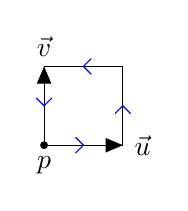
\begin{tikzpicture}
		\def\arlen{0.1};
		\fill (0,0) circle [radius=0.05cm];
		\draw (0,0) -- (1,0) -- (1,1) -- (0,1) -- cycle;
		\draw [->] (0,0) -- (1,0);
		\draw [->] (0,0) -- (0,1);
		\draw[blue] ({0.5-\arlen},{0+\arlen}) -- (0.5,0) -- ({0.5-\arlen},{0-\arlen});
		\draw[blue] ({1+\arlen},{0.5-\arlen}) -- (1,0.5) -- ({1-\arlen},{0.5-\arlen});
		\draw[blue] ({0.5+\arlen},{1+\arlen}) -- (0.5,1) -- ({0.5+\arlen},{1-\arlen});
		\draw[blue] ({0+\arlen},{0.5+\arlen}) -- (0,0.5) -- ({0-\arlen},{0.5+\arlen});
		%
		\draw (0,-0.25) node {$p$};
		\draw (1.25,0) node {$\vec{u}$};
		\draw (0,1.25) node {$\vec{v}$};
	\end{tikzpicture}
\]

\par\noindent
Even though we're taling about an operator, it's given by a tensor. $\mathcal{R}$ itself is a section of
\[
	\underbrace{T^{*}M\vphantom{\mathcal{E}_{p}}\otimes{}T^{*}M}_{\ptxt{$2$-form part}}\otimes\underbrace{\mathcal{E}_{p}\otimes\mathcal{E}_{p}}_{\hspace{-35pt}\mathrlap{\ptxt{Endomorphism part}}}
\]

\par\noindent
We're well on our way to defining the Levi-Civita connection!\n

\par\noindent
Consider a vector bundle $\mathcal{E}\to{}M$, now with a positive definite inner product on each fiber. (In the case where $\mathcal{E}=TM$, this exactly is a Riemannian metric.)\n

\defn{
	A connection $\nabla$ on $\mathcal{E}$ (with $\giprod$) is said to preserve $\giprod$ iff $\forall\gamma:[a,b]\to{}M$, parallel transport $\mathcal{P}_{\gamma}:\mathcal{E}_{\gamma(a)}\to\mathcal{E}_{\gamma(b)}$ is an isometry, i.e., $\forall{}u,v\in\mathcal{E}_{\gamma(a)}$, $\iprod{\mathcal{P}_{\gamma}(u),\mathcal{P}_{\gamma}(v)}_{\gamma(B)}=\iprod{u,v}_{\gamma(a)}$.\n
}

\prop{
	Given a vector bundle $\mathcal{E}\to{}M$, inner product $\giprod$ on each fiber, and a connection $\nabla$, the following are equivalent:
	\begin{enumerate}[label=(\alph*), leftmargin=4\parindent]
		\item $\nabla$ preserves $\giprod$.
		\item $\forall{}s,t\in\Gamma(\mathcal{E})$, $\forall{}X\in\mf{X}(M)$, $X(\iprod{s,t})=\iprod{\nabla_{X}s,t}+\iprod{s,\nabla_{X}t}$. Note that $\iprod{s,t}$ is a function on $M$, which we can differentiate with respect to $X$. We can think of this as a sort of ``product rule''.
		\item $\forall(E_{1},\ldots,E_{r})$ local orthonormal frame (which exists by Gram-Schmidt), the connection matrix $\vartheta$ is skew symmetric, i.e., $\forall{}i,j$, $\theta_{j}^{i}=-\theta_{i}^{j}$.
	\end{enumerate}\up\n
	Proof: First, we show that (b) $\Leftrightarrow$ (c). Let $(E_{1},\ldots,E_{r})$ be our local orthonormal frame. Then there are functions $f^{i},g^{j}$ such that $s=f^{i}E_{i}$ and $t=g^{j}E_{j}$. Thus, we can form $\vec{f},\vec{g}$, and by orthonormality of the frame
	\[
		\iprod{s,t}=\sum_{i=1}^{r}\sum_{j=1}^{r}f^{i}g^{j}\underbrace{\iprod{E_{i},E_{j}}}_{=\delta_{ij}}=\sum_{i=1}^{r}f^{i}g^{i}=\vec{f}\cdot\vec{g}
	\]
	Thus, with a slight abuse of notation,
	\[
		\iprod{\nabla_{X}s,t}\ptxt{``=''}(\nabla_{X}\vec{f})\cdot\vec{g}=(X(\vec{f})+\vartheta(X)\vec{f})\cdot\vec{g}
	\]
	And
	\[
		\iprod{\nabla_{X}s,t}+\iprod{s,\nabla_{X}t}=\underbrace{X(\vec{f})\cdot\vec{g}+\vec{f}\cdot{}X(\vec{g})}_{=X(\vec{f}\cdot\vec{g})=X(\iprod{s,t})}+(\vartheta(X)\vec{f})\cdot\vec{g}+\vec{f}\cdot(\vartheta(X)\vec{g})
	\]
	So the product rule holds iff $\forall{}s,t$ / $\forall\vec{f},\vec{g}$, $(\vartheta(X)\vec{f})\cdot\vec{g}+\vec{f}\cdot(\vartheta(X)\vec{g})=0$, which is true iff $\vartheta(X)$ is skew-symmetric.\nn
	In order to show (a), we just change the setting a bit. Let $\gamma:[a,b]\to{}M$ be a smooth curve. Take $V,W\in\Gamma_{\gamma}(\mathcal{E})$. We claim that, just as above, we get
	\[
		\underbrace{\iprod{\frac{DV}{dt},W}}_{\mathclap{\ptxt{a function of $t$}}}+\iprod{V,\frac{DW}{dt}}-\frac{d}{dt}\iprod{V,W}=(\vartheta(\dot\gamma)\vec{f})\cdot\vec{g}+\vec{f}\cdot(\vartheta(\dot\gamma)\vec{g})
	\]
	Assume $V$ and $W$ are parallel along $\gamma$. By definition, this means $\frac{DV}{dt}=\frac{DW}{dt}=0$. Then
	\[
		-\frac{d}{dt}\iprod{V,W}=(\vartheta(\dot\gamma)\vec{f})\cdot\vec{g}+\vec{f}\cdot(\vartheta(\dot\gamma)\vec{g})
	\]
	Well,
	\begin{align*}
		\ptxt{$\nabla$ preserves $\giprod$} & \Leftrightarrow\frac{d}{dt}\iprod{V,W}=0,\;\forall{}V,W\;\ptxt{parallel}\\
		& \Leftrightarrow(\vartheta(\dot\gamma)\vec{f})\cdot\vec{g}+\vec{f}\cdot(\vartheta(\dot\gamma)\vec{g})=0\;\ptxt{in all instances}\\
		& \Leftrightarrow\vartheta\;\ptxt{is skew symmetric}
	\end{align*}
	\proven
}

\thm{
	Let $M$ be a Riemannian manifold. Then $\exists\unique\nabla$ on $\mathcal{E}=TM\to{}M$ such that
	\begin{enumerate}[label=(\alph*),leftmargin=4\parindent]
		\item $\nabla$ preserves the Riemannian metric. \i{(This depends on the choice of Riemannian metric.)}
		\item $\forall{}X,Y\in\mf{X}(M)$, $\nabla_{X}Y-\nabla_{Y}X=\brack{X,Y}$. \i{(This does not depend on the choice of Riemannian metric.)}
	\end{enumerate}\up\n
}

\defn{
	This $\nabla$ is called the \u{Levi-Civita connection} on $M$.\n
}

\end{document}